\documentclass[10pt,t]{beamer}

% fonts
\usefonttheme{professionalfonts}
\usepackage[osf, sc]{mathpazo} % for rm
\usepackage{courier} % for mono
% \usepackage[euler-digits]{eulervm}
\usefonttheme{serif}
% more about eulervm:
% \mathrm -> rmdefault
% \mathbf -> bfdefault
% \mathsf -> sfdefault
% \mathtt -> ttdefault
% Thus, you should redefine the default text fonts before loading the eulervm package!
% redefine: \mathit, \mathbold, \mathcal

%math
\usepackage{amsmath}
\DeclareMathOperator*{\argmin}{arg\,min}
\DeclareMathOperator*{\argmax}{arg\,max}
\newcommand*\diff{\mathop{}\!\mathrm{d}}
% color
\definecolor{brown}{rgb}{0.4, 0.208, 0.192}
\definecolor{gray1}{rgb}{0.125, 0.125, 0.125}
\definecolor{gray2}{rgb}{0.157, 0.157, 0.157}
\definecolor{green2}{rgb}{0.16862745098039217,0.4,0.19607843137254902}
\definecolor{blue2}{rgb}{0,0.40784313725490196,0.6352941176470588}
\definecolor{brown2}{rgb}{0.6235294117647059,0.2901960784313726,0}

\definecolor{blue}{rgb}{0.18, 0.2, 0.529}
\definecolor{orange}{RGB}{206,117,59} % used for strong
\definecolor{green}{RGB}{49,104,108} % used for everywhere, link,...
\definecolor{red}{RGB}{133,60,66}
\definecolor{pink}{RGB}{184,86,150}



\setbeamercolor{caption name}{fg=green}

% settings for itemize and enumerate
\setbeamertemplate{itemize item}{\textbullet}
\setbeamertemplate{itemize subitem}{\bfseries --}
\setbeamertemplate{itemize subsubitem}{$\circ$}
\setbeamercolor{itemize item}{fg=green}
\setbeamercolor{itemize subitem}{fg=brown}
\setbeamercolor{itemize subsubitem}{fg=gray2}

\setbeamertemplate{enumerate item}{\arabic{enumi}.}
\setbeamertemplate{enumerate subitem}{(\roman{enumii})}
\setbeamertemplate{enumerate subsubitem}{\alph{enumiii}.}
\setbeamercolor{enumerate item}{fg=green}
\setbeamercolor{enumerate subitem}{fg=brown}
\setbeamercolor{enumerate subsubitem}{fg=gray2}
% main page style
\setbeamercolor{background canvas}{bg=white}
\setbeamercolor{normal text}{fg=black}
\setbeamertemplate{footline}[frame number]
\setbeamertemplate{navigation symbols}{}
\setbeamercolor{block title}{bg=green!90!black,fg=white}
\setbeamercolor{block body}{bg=green!10}
% frametitle
\setbeamertemplate{frametitle}
{
    \vskip 5pt
    \strut\Large\textcolor{green}{\insertframetitle}\strut
    \ifx\insertframesubtitle\empty
    \vskip-1.7ex
    \textcolor{green}{\hrule height0pt depth0.5pt \relax}
    \else
    \vskip-1ex
    \strut\small\textcolor{green}{\insertframesubtitle}\strut
    \textcolor{green}{\hrule height0pt depth0.5pt \relax}
    \fi
}
% titlepage
\setbeamertemplate{title page}
{
  \makebox[\textwidth][c]{
    \begin{minipage}[b][0.75\paperheight][c]{0.9\textwidth}
      \centering
      \huge\rm\inserttitle\\
      \Large\rm\insertsubtitle
      \vskip-1.5ex
      \textcolor{green}{\hrule height0pt depth0.8pt \relax}
      \vskip5pt
      \rm\normalsize\insertauthor
    \end{minipage}
  }

  \makebox[\textwidth][c]{
    \begin{minipage}[b][0.25\paperheight][c]{0.4\textwidth}
      \centering
      \rm\insertinstitute
      \par
      \rm\insertdate
    \end{minipage}
  }
}

\usepackage{hyperref}

% dashed underline
\usepackage{ulem}

\usepackage{booktabs}
% ********************************************************************
% tikz
% ********************************************************************
\usepackage{tikz}
\usetikzlibrary{positioning}
\usetikzlibrary{decorations.markings}
\usepackage{pgfplots}






\title{Empirical Asset Pricing \\ Problem Set $3$}
\author{Yu Zhou, HKUST}
\date{\today}


\begin{document}

\maketitle

\begin{frame}{Q1: Mean variance mathematics}
There are $N$ securities with an expected return vector $R$ and a variance covariance matrix $V$.

\begin{block}{Frontier portfolio}
The portfolio weight vector $X$ that minimize the portfolio variance given the target portfolio return $r_p$ is $V^{-1} (R \ \ell) A^{-1} (r_p \ 1)^{T}$.

\vskip 0.5\baselineskip
\textit{Proof.}
\begin{equation*}
\begin{split}
\mathcal{L} = & X^T V X + \pi_1 (r_p - X^TR) + \pi_2 (1 - X^T\ell) \\
\text{\scriptsize F.O.C.:\ } & 2 VX - \pi_1 R - \pi_2 \ell = 0 \\
\Rightarrow & X = 1/2 V^{-1} (R \ \ell) (\pi_1 \ \pi_2)^T \\
\text{\scriptsize Constriant:\ }& 1/2 (\pi_1 \ \pi_2) (R \ \ell)^T V^{-1} (R \ \ell) = (r_p \ 1) \\
\Rightarrow & (\pi_1 \ \pi_2) = 2 (r_p \ 1) A^{-1} \text{ where } A = (R \ \ell)^T V^{-1} (R \ \ell)\\
\Rightarrow & X = V^{-1} (R \ \ell) A^{-1} (r_p \ 1)^{T}
\end{split}
\end{equation*}
\end{block}
\end{frame}




\begin{frame}{Q1: Mean variance mathematics (cont'd)}
\begin{block}{Orthogonal portfolio}
Given a mean-variance frontier portfolio with expected return $r_p$, the expected return on the orthogonal portfolio is $r_z = (a - b r_p)/(b - c r_p)$.

\vskip 0.5\baselineskip
\textit{Proof.}
\begin{equation*}
\begin{split}
& X_p^T V X_z = 0 \\
\Leftrightarrow & (r_p \ 1) A^{-1} (r_z \ 1)^T = 0 \\
\Rightarrow & r_z = \frac{a - b r_p}{b - c r_p} \\
\text{ where } & A = \left[\begin{array}{cc}a & b \\ b & c\end{array}\right], A^{-1} = \frac{1}{ac - b^2}\left[\begin{array}{cc}c & -b \\ -b & a\end{array}\right]
\end{split}
\end{equation*}
\end{block}
\end{frame}


\begin{frame}{Q1: Mean variance mathematics (cont'd)}
\begin{block}{Tangency portfolio}
Suppose we have a risk-free asset with expected return $r_f$. The expected return on the tangency portfolio is $r_{\text{tangency}} = (a - b r_f)/(b - c r_f)$.
\end{block}

\begin{block}{Global minimum variance portfolio}
The expected return on the global minimum portfolio is $r_g = b/c$.

\vskip 0.5\baselineskip
\textit{Proof.}
\begin{equation*}
\begin{split}
& \min_{X} X^T V X \\
\Leftrightarrow & \min_{r_g} (r_g \ 1) A^{-1} (r_g \ 1)^T = \frac{1}{ac - b^2} (c r_g^2 - 2br_g + a) \\
\Rightarrow & r_g = \frac{b}{c}
\end{split}
\end{equation*}
\end{block}
\end{frame}



\begin{frame}{Q2: Data source}
\begin{itemize}
  \item Data source: \href{https://mba.tuck.dartmouth.edu/pages/faculty/ken.french/data_library.html}{\dashuline{Prof. Kenneth French's website}}.
  \begin{itemize}
    \item $10$ industry portfolios constructed at the end of June.
    \item value weighted monthly return from 1926/07--2020/07.
  \end{itemize}
  \item Let the risk-free rate be $0.33\%$ per month.
\end{itemize}
\end{frame}


\begin{frame}{Q2: MVP \& TP}
\begin{table}
\begin{tabular}{lcc}
\toprule
Industry & $X_g$ & $X_{\text{tangency}}$ \\
\cmidrule{1-3}
NoDur & $0.75$ & $0.74$\\
Durbl & $-0.07$ & $0.09$\\
Manuf & $-0.11$ & $-0.17$\\
Enrgy & $0.18$ & $0.21$\\
HiTec & $-0.1$ & $0.13$\\
Telcm & $0.54$ & $0.27$\\
Shops & $-0.05$ & $0.06$\\
Hlth & $0.09$ & $0.37$\\
Utils & $0.1$ & $0.01$\\
Other & $-0.33$ & $-0.72$\\
\cmidrule{1-3}
mean & $0.88$ & $1.05$ \\
std & $3.77 $& $4.28$ \\
\bottomrule
\end{tabular}
\caption{Both the global minimum variance portfolio and tangency portfolio longs non-durables, energy, telecom, healthcare and utilities, and shorts manufacturing and others. And, the global minimum variance portfolio longs more telecom and utilities.}
\end{table}
\end{frame}


\begin{frame}{Q2: Efficient frontier}
\begin{figure}[h!]
\centering
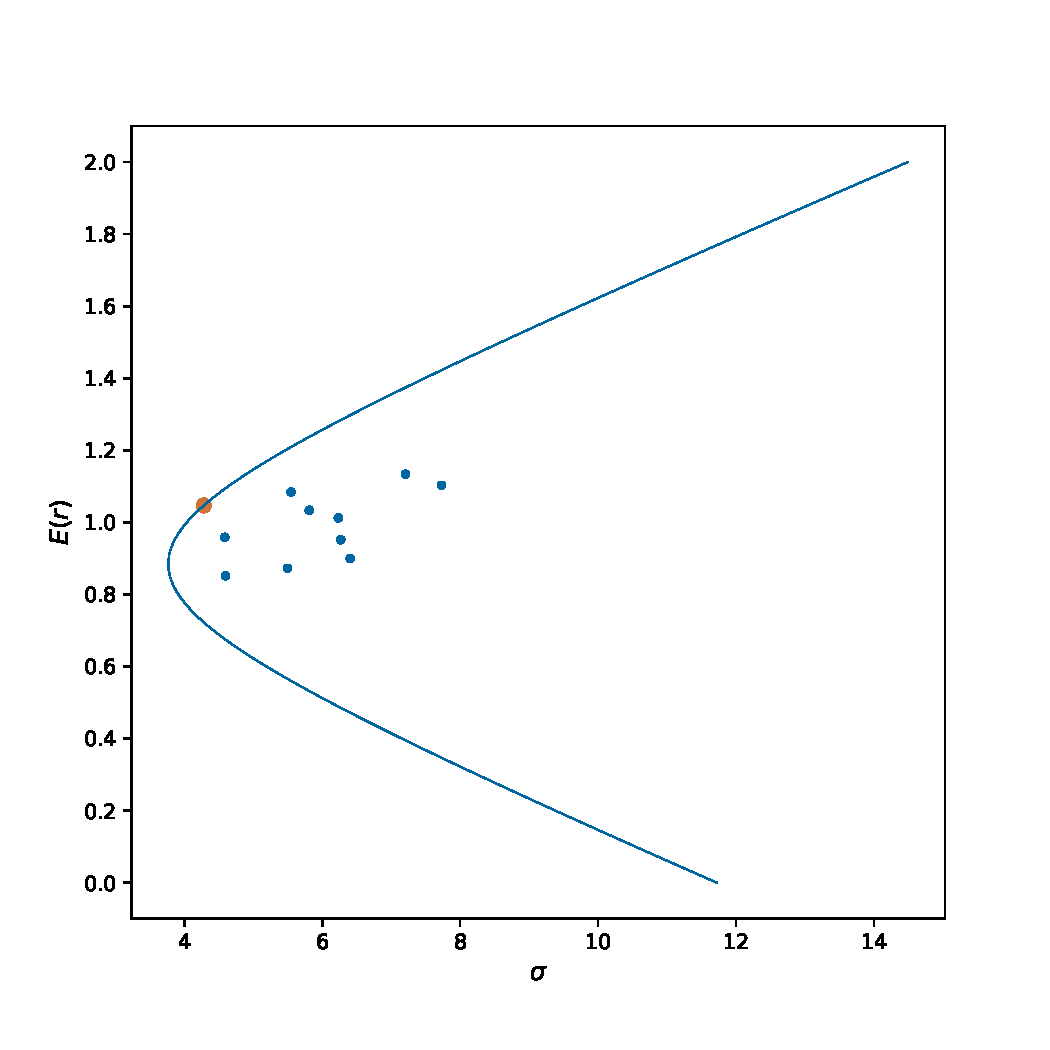
\includegraphics[width=0.5\linewidth]{q2fig1.pdf}
\caption{This figure plots the efficient frontier constructed from these $10$ industries. It is a parabola because these ten portfolios are not perfectly correlated. Some portfolios constructed based on them have less standard deviations.}
\end{figure}
\end{frame}


\begin{frame}{Q2: Monte Carlo simulation}
\begin{itemize}
  \item Steps:
  \begin{itemize}
    \item Historical real returns $\rightarrow$ $R^\circ$, $V^\circ$;
    \item $N(R^\circ, V^\circ) \rightarrow$ sample $\rightarrow$ $\hat{R}$, $\hat{V}$ $\rightarrow$ $\hat{X}_g$, $\hat{X}_{\text{tangency}}$;
    \item Apply $\hat{X}$ to $R^\circ$, $V^{\circ}$.
  \end{itemize}
\end{itemize}
\end{frame}

\begin{frame}{Q2: Monte Carlo simulation (cont'd)}
\begin{figure}[h!]
\centering
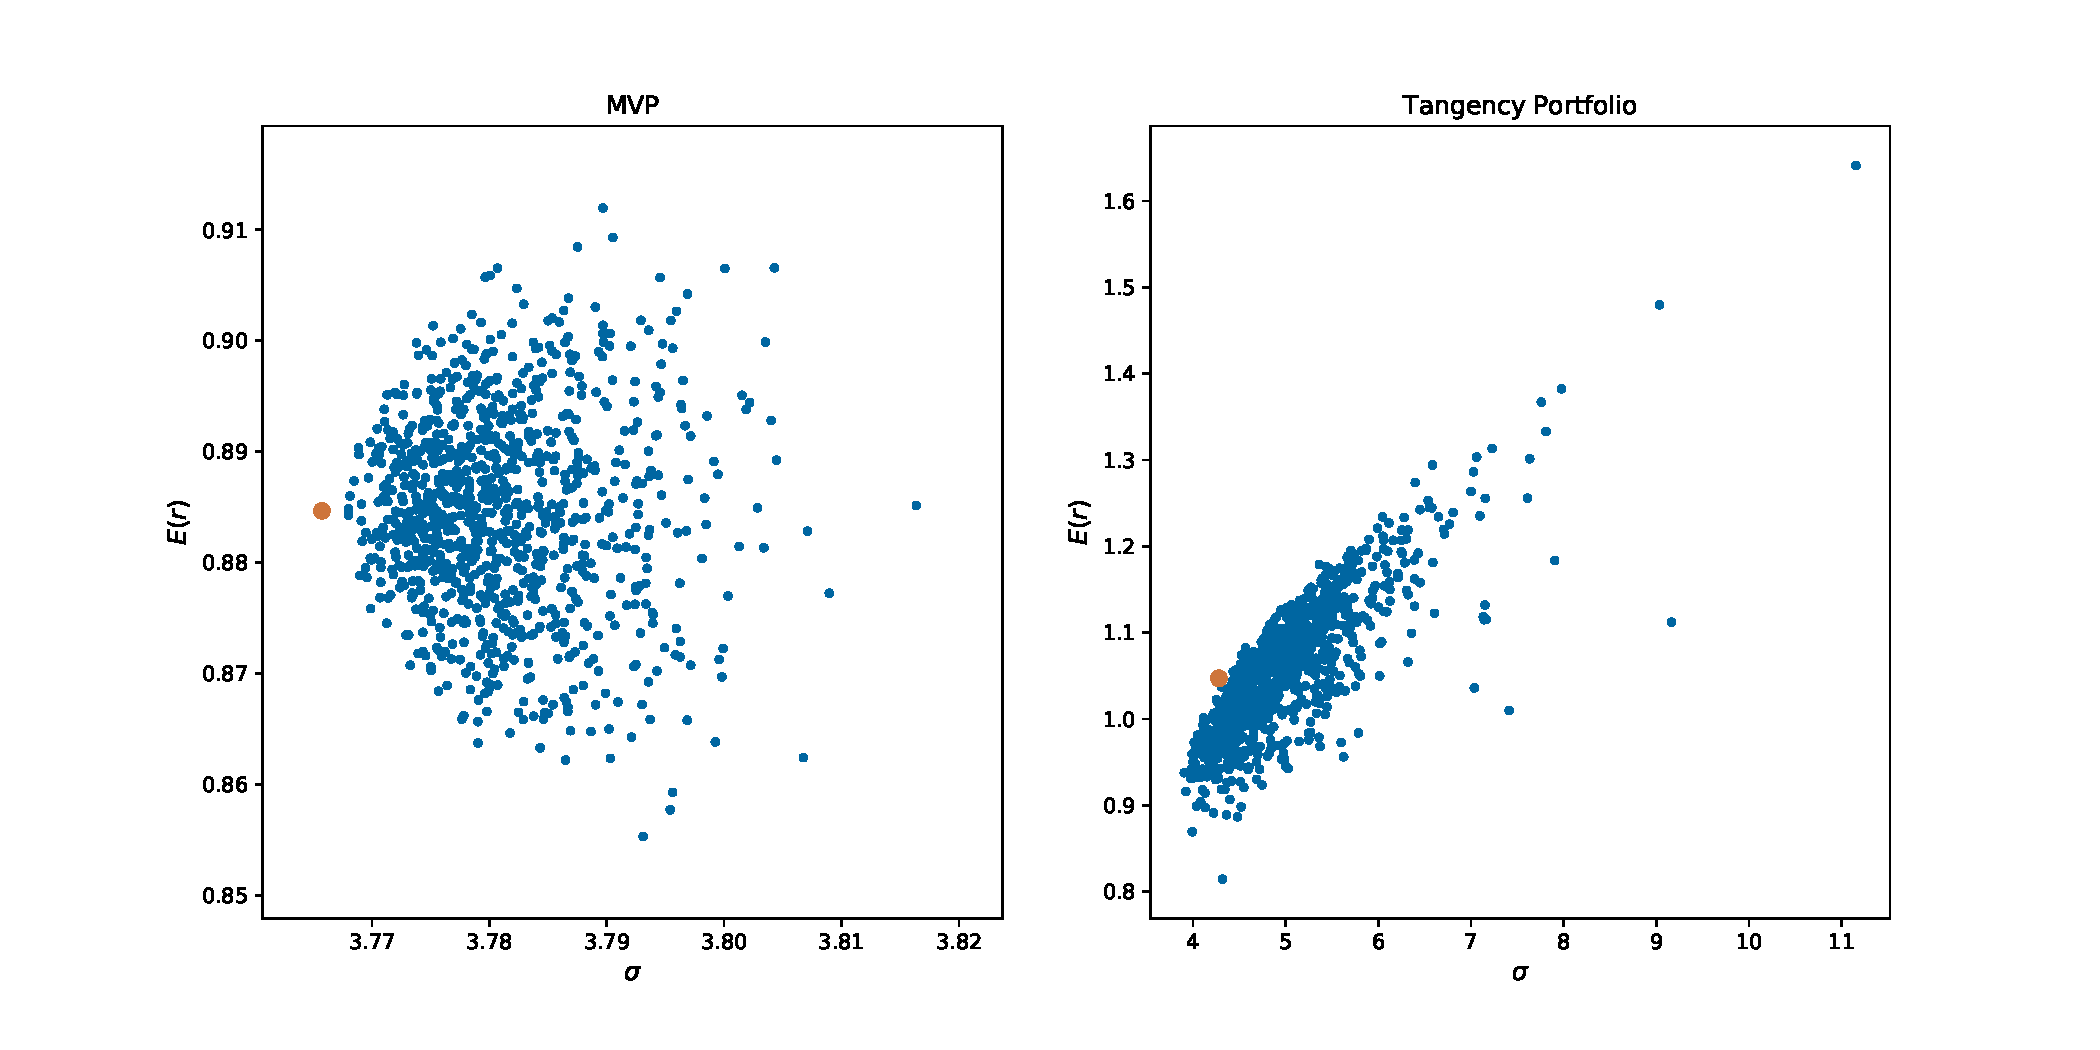
\includegraphics[width=\linewidth]{q2fig2.pdf}
\caption{The global minimum variance portfolio is estimated with less error. This results from the fact that $\hat{X}_g = \hat{V}^{-1} \ell / c$ only depends on the estimate of the second moment, where $c = \ell^T \hat{V}^{-1} \ell$. But the tangency portfolio also relies on the esimate of the first moment.}
\end{figure}
\end{frame}



\begin{frame}{Q2: Block bootstrap simulation}
\begin{itemize}
  \item Steps:
  \begin{itemize}
    \item Historical real returns $\rightarrow$ empirical distribution;
    \item Select a number between $1$ to $T$ for $T$ times $\rightarrow$ sample $\rightarrow$ $\hat{R}$, $\hat{V}$ $\rightarrow$ $\hat{X}_g$, $\hat{X}_{\text{tangency}}$;
    \item Apply $\hat{X}$ to $R^\circ$, $V^{\circ}$.
  \end{itemize}
\end{itemize}
\end{frame}


\begin{frame}{Q2: Block bootstrap simulation (cont'd)}
\begin{figure}[h!]
\centering
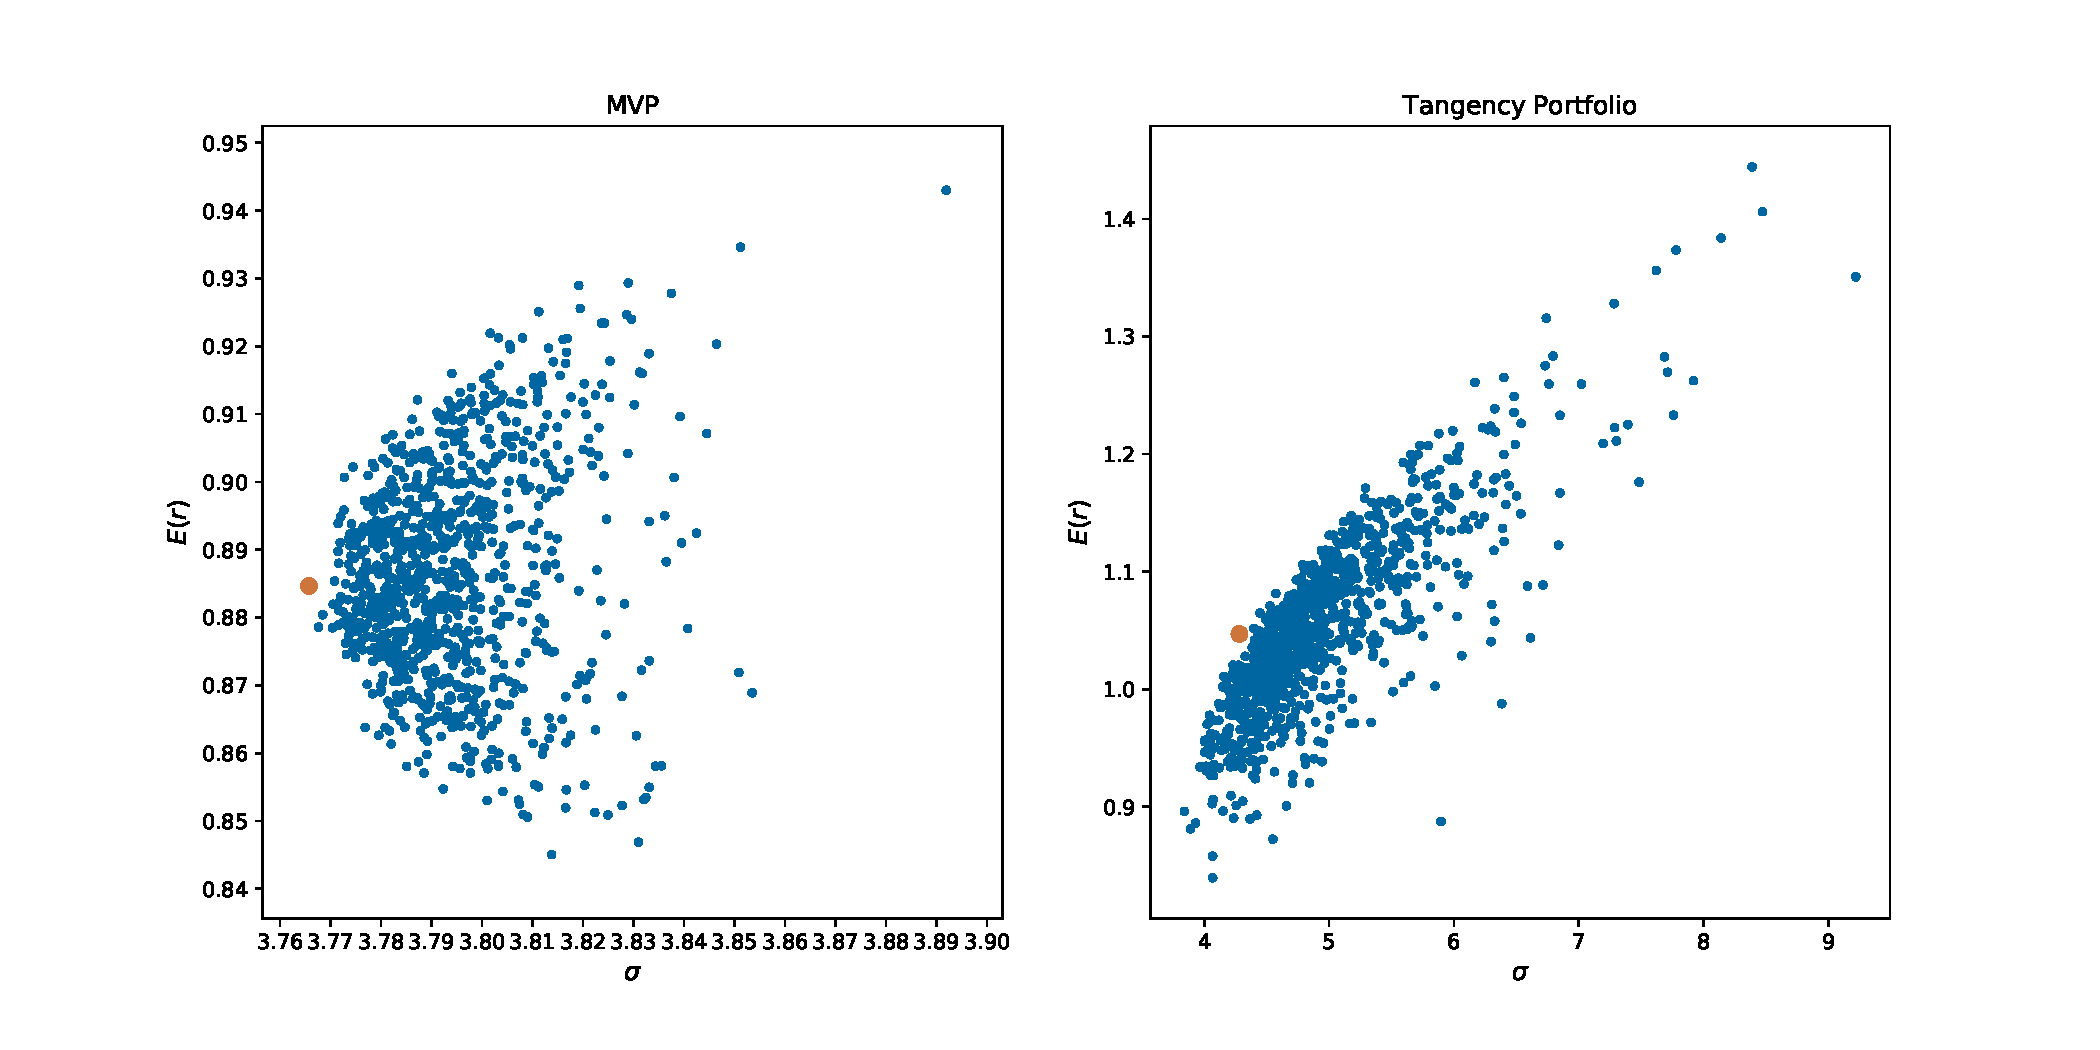
\includegraphics[width=\linewidth]{q2fig3.pdf}
\caption{The global minimum variance portfolio is still estimated with less error. Compared with the Monte Carlo simulation, the block bootstrap simulation features more estimation error. The reason is that the block bootstrap simulation puts less restrictions on the family of estimated distributions (i.e., nonparametric).}
\end{figure}
\end{frame}


\begin{frame}{Q2: A simple asset pricing test}
\begin{figure}[h!]
\centering
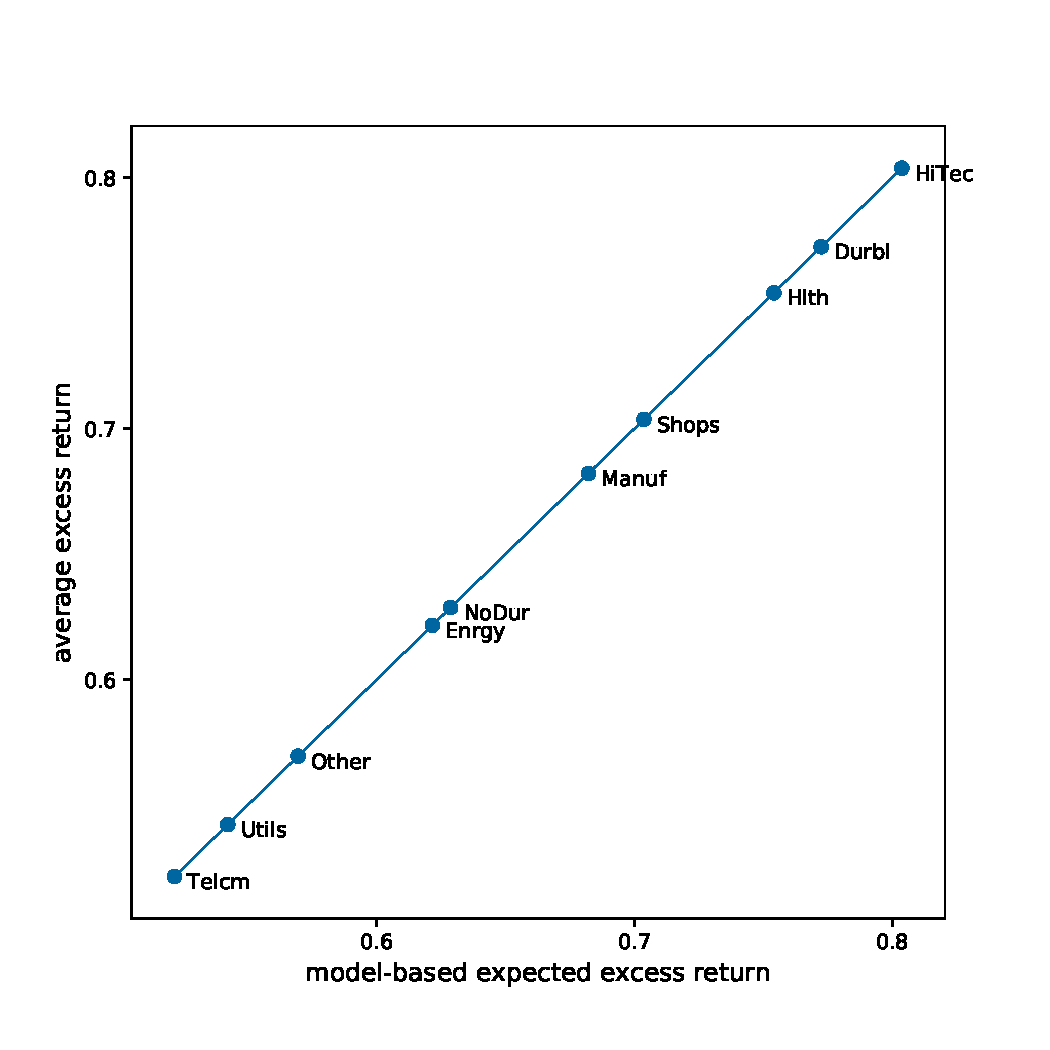
\includegraphics[width=0.5\linewidth]{q2fig4.pdf}
\caption{Running a regression of industry portfolio's excess return on the tangency portfolio's excess return, I find that $\hat{\alpha} = 0$ and average excess returns coincide with model-based expected excess returns. This result is not surprising, because beta pricing formula is a purely mathematical equation which alway holds.}
\end{figure}
\end{frame}

\begin{frame}{Q2: An out-of-sample asset pricing test}
\begin{table}
\begin{tabular}{lcc}
\toprule
Industry & $\hat{\alpha}_i$ & $\hat{\beta}_i$ \\
\cmidrule{1-3}
NoDur & $0.43$ & $0.41$\\
Durbl & $0.07$ & $0.69$\\
Manuf & $0.25$ & $0.53$\\
Enrgy & $0.19$ & $0.53$\\
HiTec & $0.08$ & $0.88$\\
Telcm & $0.2$ & $0.56$\\
Shops & $0.34$ & $0.53$\\
Hlth & $0.22$ & $0.65$\\
Utils & $0.44$ & $0.18$\\
Other & $0.23$ & $0.48$\\
\bottomrule
\end{tabular}
\caption{Estimating the weight for the tangency portfolio using data before 1973 and running an out-of-sample (i.e., after 1973) regression, I find that for all industies $\hat{\alpha}_i > 0$.}
\end{table}
\end{frame}

\begin{frame}{Q2: An out-of-sample asset pricing test (cont'd)}
\begin{figure}[h!]
\centering
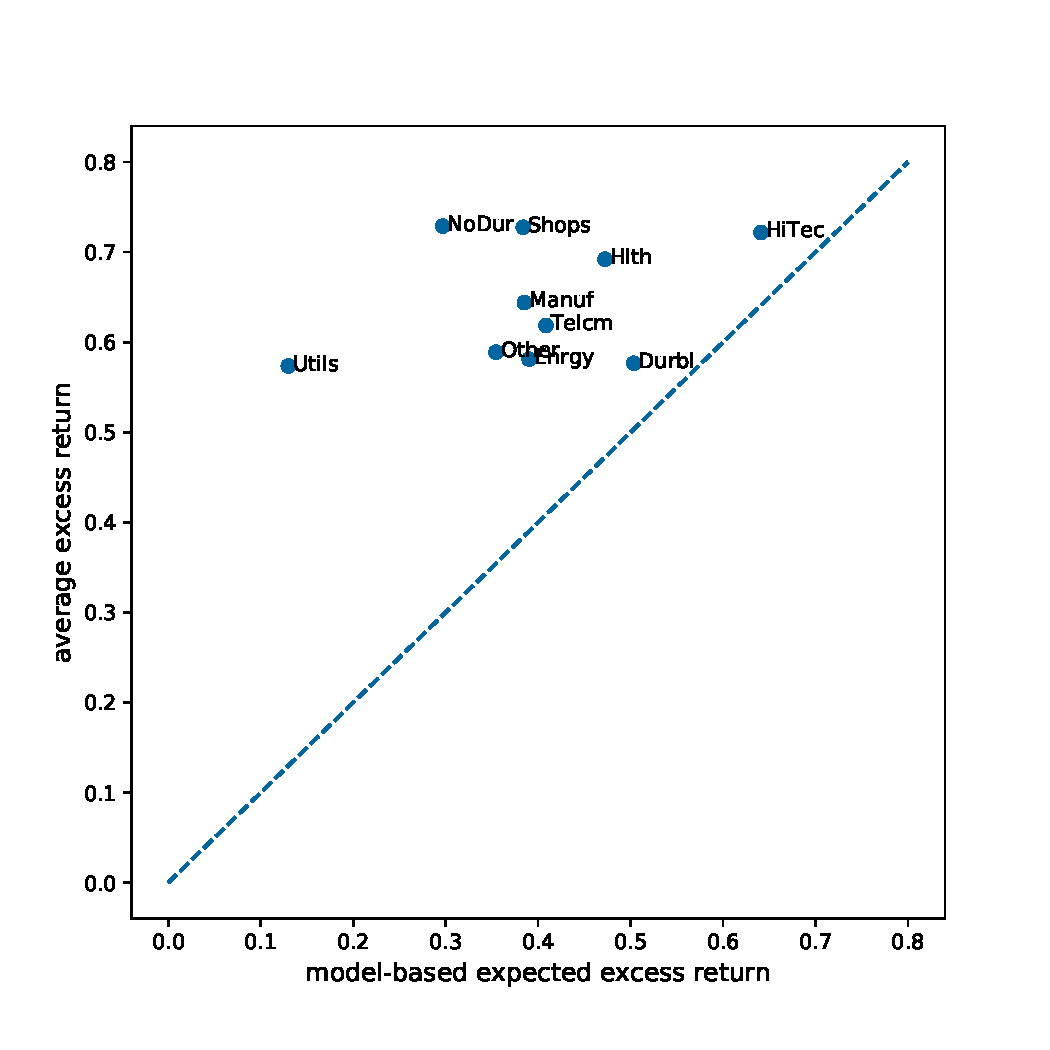
\includegraphics[width=0.5\linewidth]{q2fig5.pdf}
\caption{For all industies, average excess returns are larger than model-based expected excess returns after 1973. This result implies that there is a structural difference of mean and variance of returns between these two periods. The distribution of returns and the weight for the tangency portfolio are time-varying.}
\end{figure}
\end{frame}



























\end{document}

